\chapter{Bildvorverarbeitung}

Bevor nach der Aufnahme des Bildes nach Linien gesucht werden kann, muss das Bild noch entzerrt, gefiltert und binarisiert werden. 

\section{Bildentzerrung}

Der goße Vorteil des Fischaugenobjektivs ist es, Bereiche in größerer Entfernung in alle Richtungen  wahrnehmen zu können. Jedoch ist es gerade für die Approximation der Fahrbahnmarkierungen zur Erstellung einer Weltkarte und der Regelung des Autos sinnvoll, dessen Verzerrung zurückzurechnen. Dazu wurde sich in Matlab wie in (REFERENZ AUF GRUNDLAGEN KAMERAMODELL) beschrieben der OcamCalib-Toolbox bedient. Zuvor erfolgt außerdem eine Umwandlung in ein Graustufenbild, da wir die Farbinformation der Rohdaten nicht mit verarbeiten und sowohl die Toolbox als auch die Filter nur mit Schwarz-Weiß-Bildern, also einer Matrix deren Einträge die Helligkeitswerte der Pixel darstellt, arbeiten können. 

\begin{figure}[H] % [htb]
  \centering
  \subfloat[][]{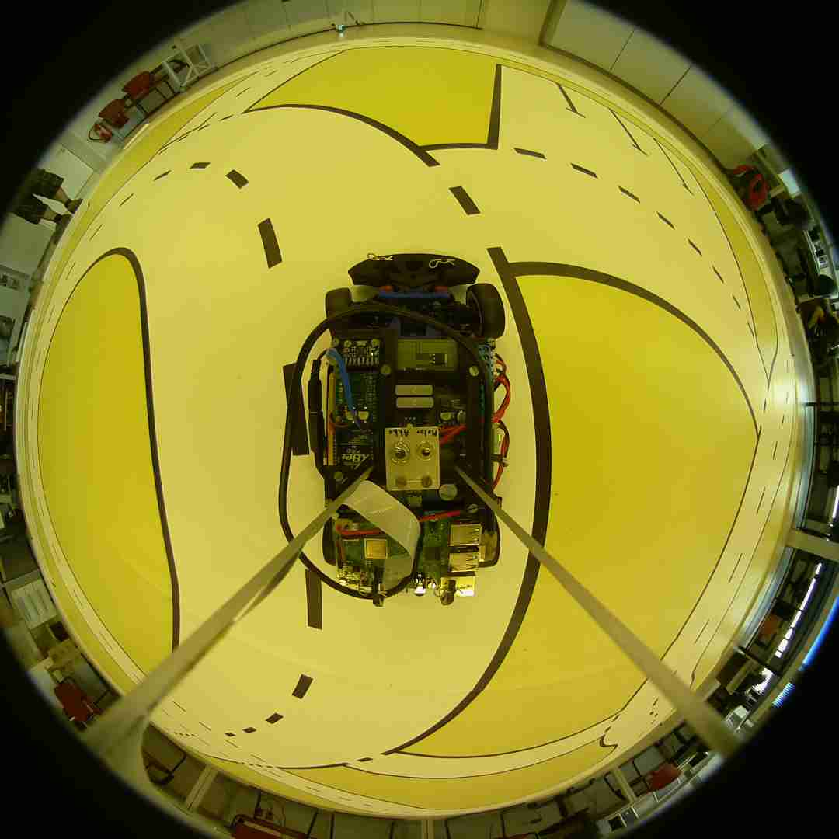
\includegraphics[width=0.45\textwidth]{bildvorverarbeitung_fischauge.png}}
  \quad
  \subfloat[][]{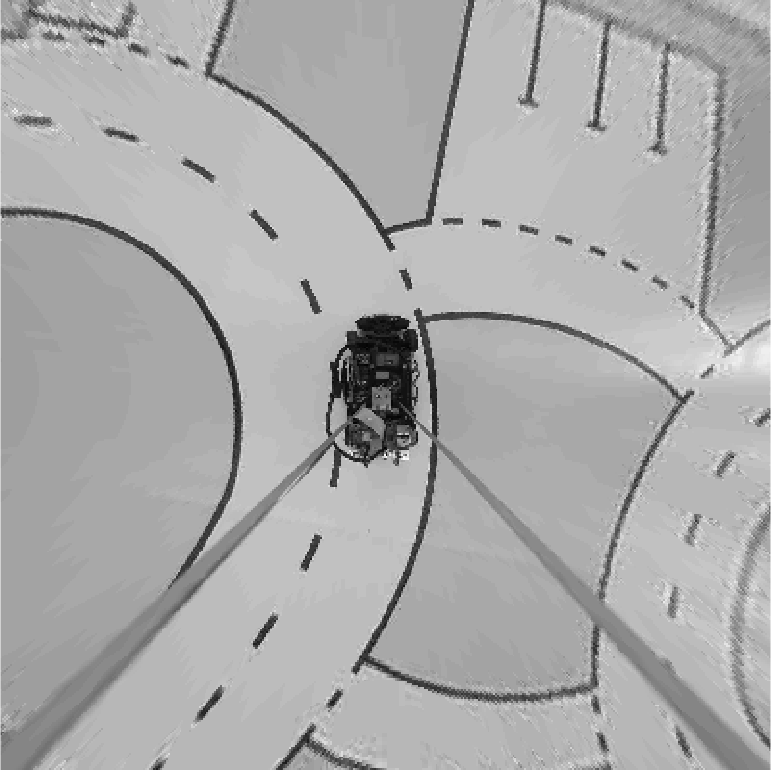
\includegraphics[width=0.45\textwidth]{bildvorverarbeitung_entzerrt.png}}
%  \includegraphics[width=0.9\textwidth]{bildvorverarbeitung_entzerren.png}
  \caption{verzerrtes Rohbild (a) und entzerrtes Graustufenbild (b) einer Momentaufnahme im Parcour}
\label{fig:bildvorverarbeitung_entzerren}
\end{figure} 

In~\ref{fig:bildvorverarbeitung_entzerren} ist zu sehen, wie das Bild original (links) und nach der Entzerrung (rechts) aussieht. Im entzerrten Bild fällt auf, dass zum Rand die Auflösung durch die Transformation immer schlechter wird. Daher haben wir den Bildausschnitt so weit begrenzt, sodass nach der Filterung die Linien noch akzeptabel erkennbar waren.

\section{Filterung}




\section{Binarisierung}

